% !TEX root = ./dissertation.tex

\section{Introduction}

This thesis is a small exploration into the interconnected and mysterious worlds
of mathematical logic and computation. Since the advent of the fields in the
early 20th Century, links have been found in unusual places and both fields have
provided insight into the other. There are two primary focal points of this
thesis: the unification of disparate areas in mathematical logic and computing
via category theory, an offshoot of abstract algebra; and the rigorous
formalisation of mathematics within modern theorem provers. More precisely, a
particular theorem within category theory will be proven within the theorem
prover Agda and its applications will be explored, with a new application
provided in the context of the untyped $\lambda$-calculus. The theorem that will
be explored within this thesis is Lawvere's fixed point theorem discovered by
William Lawvere in 1969 in \textit{Diagonal Arguments and Cartesian Closed
Categories} \cite{lawvere1969diagonal}. Lawvere's fixed point theorem is a
statement within the context of cartesian closed categories, categories which
play a crucial role within the study of computation and logic. Interested was
somewhat renewed in Lawvere's theorem in 2003 after a review paper published by
Noson Yanofsky \cite{yanofsky2003universal} detailed how many common paradoxes
and results in computing and mathematical logic could be brought within the
framework of the theorem. Lawvere's fixed point theorem is a categorical
abstraction of the familiar class of \textit{diagonal arguments} employed
throughout computer science and mathematics. The decision to formalise Lawvere's
fixed point theorem within a theorem prover is not incidental; many of the
theorems abstracted by the theorem play an important role in the problem of
providing a formal foundation in which to do mathematics.

The primary contributions of this thesis are: a formalisation of Lawvere's fixed
point theorem within the theorem prover Agda with additional proofs in the
theory of cartesian closed categories; a novel application of Lawvere's fixed
point theorem within the context of the untyped $\lambda$-calculus; and a
formalisation within Agda of a category of small types with presentations of
Cantor's Theorem. Given the attempts of this thesis to incoporate a large amount
of related yet distinct fields together the contextual history behind the
primary areas must be outlined. What follows is a blurred and idealistic
exposition of background of 20$^{\textrm{th}}$ century mathematical logic.

\theoremstyle{definition}
\newtheorem{theorem}{Theorem}
\newtheorem*{theorem*}{Theorem}
\newtheorem{definition}{Definition}

\section{Foundations of Mathematical Logic and Computation}

\subsection{Cantor's Theorem}

The story begins slightly before the advent of the 20$^{\textrm{th}}$ century
with the German Mathematician Georg Cantor. Cantor (1845 - 1918) is considered
the father of set theory with his proofs of the differing cardinalities of the
real and natural numbers and theory of ordinals. A major piece of work by Cantor
was his eponymous theorem \cite{cantor1892ueber}, published in 1892, that the
cardinality of a set is strictly smaller than the cardinality of its powerset.
Cantor's proof of this theorem made use of a so-called \textit{diagonal
argument}, one of the first of its kind which, repeated through time in
different fields, was abstracted by Lawvere to give his fixed point theorem in
category theory subsuming previous instances. Cantor's theorem proceeds has
follows:

\begin{theorem*}[\textbf{Cantor's Theorem}]
    Let $f$ be a function from a set $A$ to its powerset $\mathcal{P}(A)$. Then
    $f$ is not a surjective function.
\end{theorem*}

\begin{proof}
    Aiming for a contradiction assume $f$ is surjective. Consider the set $B =
    \{ a \in A \: | \: a \not\in f(a) \}$. Therefore there exists a $b \in A$
    such that $f(b)=B$. By definition $f(b) = B$ and therefore $b \not\in B$.
    However, $b \not\in f(b)$ implies $b \in B$. Contradiction.
\end{proof}

The name \textit{diagonal theorem} comes from an earlier proof by Cantor of the
uncountability of the real numbers. This was done by assuming an enumeration of
the set of infinite sequences of binary digits which are in correspondence with
the real numbers, and considering this as a table, see Figure
\ref{fig:diagonal}. The proof then proceeds by going along the diagonal of the
table flipping the $n^{th}$ digit of the $n^{th}$ number going down the table to
produce a new real number not in the table. The repetition of the argument in
two places in the definition yields a familiar structure repeated in many
theorems in mathematical logic known as \textit{diagonal arguments}. The set

\begin{figure}[h]
    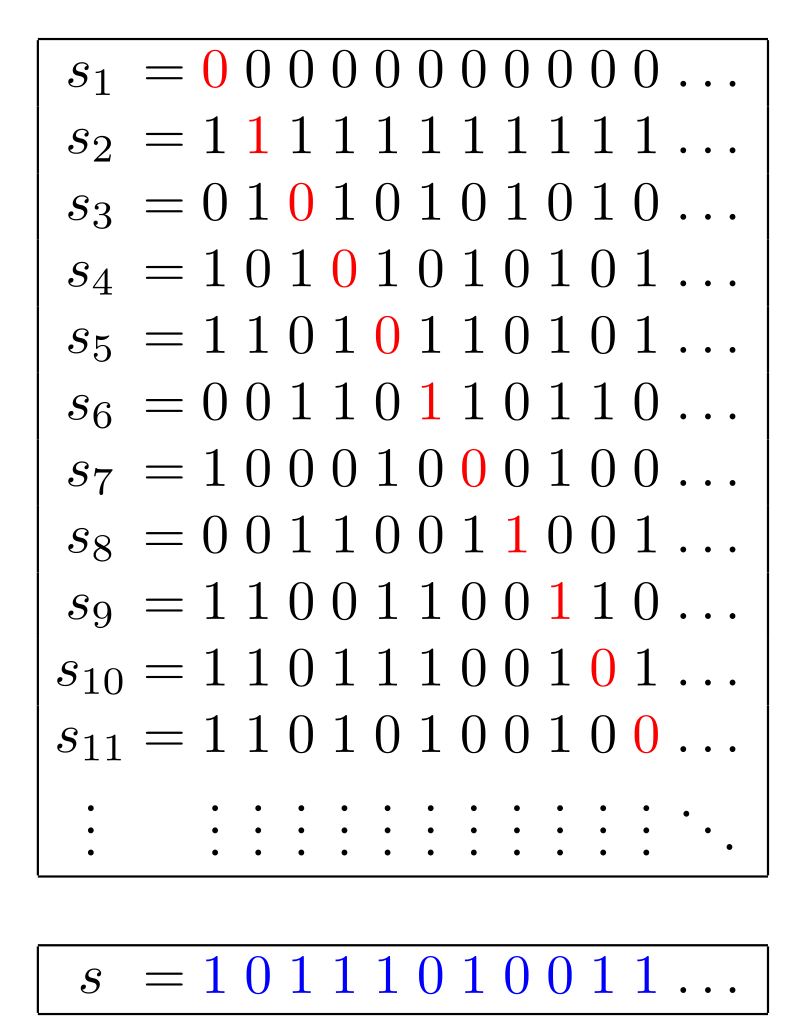
\includegraphics[width=5cm]{diagonal.png}
    \centering
    \caption{Cantor's Diagonal Argument Illustrated }
    \label{fig:diagonal}
\end{figure}

\subsection{Russell's Paradox}
Cantor, in founding set theory as a field of study, introduced his na{\"i}ve set
theory \cite{Cantor:1874} as a foundation in which to do mathematics. The
na{\"i}vity of Cantor's foundations rested in the \textbf{Axiom of Unrestricted
Comprehension}, adapted from Gottlob Frege's \textbf{Basic Law \RNum{5}}
\cite{frege1884grundlagen} where $w_{1}$, \ldots , $w_{n}$ ranges over the words
of the language of sets which states that that for all predicates (functions
that return a boolean value), $\varphi$, there exists a set, $B$, whose elements
exactly satisfy $\varphi$.

\begin{definition}[\textbf{Axiom of Unrestricted Comprehension}]
    {\large
    \begin{align*}
        \forall \varphi \; \forall w_{1}, \cdots , w_{n} \; \exists \, B.  \textrm{ such that }
        \forall x  \; (x \in B \textrm{ iff. }  \varphi(x, w_{1},\cdots,w_{2} ))
    \end{align*}
    }%
\end{definition}

. This lead to perhaps the first signifcant result in the foundations of
mathematics in the 20$^{\textrm{th}}$ century, Russell's paradox. Betrand Russell (1872-1970),
an English polymath, showed in \textit{The Principles of Mathematics}
\cite{russell1903principles} written with Alfred Whitehead in 1903 that, in
classical logic, the axiom of unrestricted comprehension leads to a
contradiction.

\begin{theorem}[\textbf{Na{\"i}ve set theory is inconsistent}]
\end{theorem}

\begin{proof}
    Consider the predicate
    \begin{align*}
        \varphi(x) = x \not\in x
    \end{align*}
    By the \textbf{Axiom of Unrestricted Comprehension} there is a set $X$ such
    that all $x \in X$ satisfy $\varphi$. Aiming for a contradiction, assume
    $X \in X$. By definition of $\varphi$, $X \not\in X$. Contradiction.
\end{proof}

This proof shares the similar diagonal style argument where $x$ appears in the
postive and negative positions of the set membership relation $\in$. In modern
set theories, this is disposed of in favour of an axiom of restricted
comprehension, where all predicates must be defined on an already existing set.
For a set theory to be consistent it must therefore reject the \textbf{Axiom of
Restricted Comprehension}. This in turn prevents the existence of a set of all
sets from being considered as this must contain itself, something which is not
supported by restricted comprehension schemes. This result is relevant to both
prongs of this thesis. Russell's paradox presented a blow to the hoped
foundations of mathematics. Various systems were designed to provide a more
secure foundation of mathematics as a result of Russell's paradox. Russell
himself created the first theories of types in his \textit{Principia
Mathematica} \cite{russell25} to combat this with various other foundational
theories being presented, including set theoretic foundations such as
Zermelo-Fraenkel set theory (ZFC) and Von-Neumann-Bernays-G{\"o}del set theory
(NBG) which reject the axiom of unrestricted comprehension. Yanofsky
\cite{yanofsky2003universal} shows how Russell's paradox can be brought within
the framework of Lawvere's fixed point theorem.

\subsection{Computability}
Shortly after the work of Cantor and Russell, the field of theoretical computer
science was birthed by attempts to answer the \ent{} (decision
problem), a challenge by David Hilbert \cite{hilbert1928theoretische} which required the formalisation of the
notion of algorithm.

\subsubsection{\ent}

Devised in 1928 by Hilbert, the \ent asked for an effective procedure or
algorithm which, on an input of a statement in first-order logic plus a finite
numbers of axioms, could determine its validity in all structures statisfying
the axioms. Before an answer could be given, the notion of algorithm had to be
formalised. This was done in the 1930s independently by Alonzo Church and Alan
Turing. Turing's formalisation \cite{turing1937computable} known as Turing
Machines, aimed to capture directly the notion of algorithm. Turing provided a
negative answer to this question by establishing the existence of undecidable
problems such as the Halting problem and confirming the \ent as one of these
undecidable problems. Turing's proof of the existence of undecidable problems
and his proof of the Halting problem resemble closely the proof of Cantor's
theorem being diagonalisation arguments. Yanofsky \cite{yanofsky2003universal}
also  shows how both proofs can be understood through the lens of Lawvere's
fixed point theorem by considering the category of computable universes or
objects which "support computation"

\subsubsection{$\lambda$-calculus}
Instead of capturing directly the notion of computability, Alonzo Church's
formalisation was focused on formalising more precisely the notion of a
function.  Church's formulation, the $\lambda$-calculus \cite{church1932set}, is
a formal system consisting of the operations of abstraction and application
using variable binding and substitution. Church showed that the
$\lambda$-calculus had an notion of $\lambda$-definability
\cite{church1936unsolvable} which was equivalent to the class of general
recursive functions \cite{kleene1936general} as defined by G{\"o}del and
clarified by Kleene, another model of computation.  Church also provided a
negative answer to the \ent. The $\lambda$-calculus has applications beyond that
of providing a negative answer to the \ent.

The $\lambda$-calculus consists of a set of inductively defined terms and
rewriting rules governing how to compute with them. In the definitions that
follow $s$ and $t$ range over $\lambda$-terms and $x$ ranges over variable
names.

\begin{definition}[\textbf{The set} $\bm{\Lambda}$ \textbf{of}
    $\bm{\lambda}$\textbf{-terms}]
    \begin{gather*}
        x \in \Lambda \\
        s \in \Lambda \; \land \; t \in \Lambda \implies (s \; t) \in \Lambda \\
        s \in \Lambda \; \implies \lambda x . s \in \Lambda
    \end{gather*}
\end{definition}

$(s \: t)$ denotes the application of $s$ to $t$ and $\lambda x . s $ denotes
the \textit{capture} or \textit{binding} of the variable $x$ in term $s$, known
as a $\lambda$-abtraction. Intuitively, application of a term to a
$\lambda$-abstraction, when considered as a computation, should replace all
instances of the abstracted variable with the term being applied a process known
as substitution. This computation is known as $\beta$-reduction.


\begin{definition}[$\bm{\beta}$\textbf{-reduction}] A term $t$ applied to
    $\lambda$-abstraction $(\lambda x . s \; t)$, $\beta$\textit{-reduces} to
    $s[t/x]$ denoting the substitution of $t$ for $x$ in $s$ written
    \begin{align*}
        (\lambda x . s \; t) \rightarrow_{\beta} s[t/x]
    \end{align*}
\end{definition}
With this notion of reduction an equational theory can be produced capturing the
notion of equivalence under $\beta$-reduction which will be referred to as
$\lambda\beta$.

The $\lambda$-calculus originally arose from Church's desire to provide a foundation
for logic, a desire also shared by another American Logician, Haskell Curry. In
the 1920s and 1930s, Curry worked on a foundation of logic extremely similar to
the $\lambda$-calculus, his theory of combinators \cite{curry1930grundlagen}.
Combinatory logic, as defined by Curry, was in correspondence with the
$\lambda$-calculus. In 1934 Curry observed that, if types were assigned to the
domains and comdomains of his combinators, the types matched the axioms of
intuitionistic implicational logic \cite{curry1934functionality}. This
observation proved to be the beginning of theorem provers as they are in their
current state.

\subsection{Curry-Howard Correspondence}
Curry's combinatory logic and Church's $\lambda$-calculus, when viewed as a
system for logic, proved to be inconsistent as shown by Kleene and Rosser
\cite{kleene1935inconsistency} and again by Curry using his Paradoxical
Combinator \cite{curry1941paradox}. To remedy this inconsistency both Curry and
Church restricted their logical systems with types giving typed combinatory logic
and the simply typed $\lambda$-calculus. Further to Curry's aformentioned
observation made of typed combinatory logic, in the 1960s William Alvin Howard
made a further observation that the typing rules of the simply
$\lambda$-calculus corresponded to laws of inference for intuitionistic style
natural deduction \cite{howard1980formulae}. This lead to the conclusion that
every system in formal logic has a corresponding computational calculi with a
specific type system named the Curry-Howard correspondence. The relation of
computational calculi to \textit{intuitionistic} logic is an interesting one.
Intuitionistic logics are a class of logics that reject some common principles
of classical logic namely the Law of Excluded Middle (LEM), $(\vdash p \lor \lnot p)$,
and Double Negation Elimination (DNE) $(\lnot \lnot p \vdash p)$. Intuitionistic Logic
is highly related to the philosophical position of mathematical constructivism.
Mathematical constructivism places a higher burden on proof when positing the
existence of mathematical strucures and demands that a mathematical object be
explicitly constructed.  Both LEM and DNE are able to prove the existence of
objects that have not been explicitly constructed through the use of proof by
contradiction. Constructivism can be seen as a natural counterpart the
philophical position of intuitionism which asserts that mathematics is an
entirely human activity that arises from our mental faculty, contrary to
platonsism which makes stronger ontological claims about the objective status of
mathematical structures. The effectiveness of the Curry-Howard correspondence in
formalising and mechanizing mathematics gives some credence to this theory and
the act of theorem proving can be seen as a continuation of the underlying
causes of intuitionistic movements.

\section{History of Theorem Proving}
The Curry-Howard correspondence provided a computational interpretation of the
notion of proof. Providing a proof of a theorem corresponded to a program that
inhabited a given type. Type systems in computation had largely grown with the
theory of programming languages. Types were intended to check that a program, to
some degree, behaved as intended. It was understood that the comprehensive type
systems and their associated checkers could be used to check the validity of
proofs in mathematics. With the advent of physical computers this provided hope
that a more methodical approach to mathematics that eliminated the uncertainty
around new proofs would be achieved.
\subsection{Automath}
The first computational system to exploit the Curry-Howard correspondence to act as
a theorem prover was Automath in 1967, slighty before Howard's explicit
observation of the Curry-Howard correspondence. Automath (automating
mathematics) was designed by Dutch Mathematician, Nicolaas Govert de Brujin (of
index fame) \cite{de1983automath}, who independently observed the Curry-Howard correspondence.
Automath was a typed programming language providing inbuilt support for variable
binding, substitution and application of judgemental equalities. This has been
a common feature of proof-assistants since and is the defining features of
a set of computational calculi known as \textit{logical frameworks}. Users could
define their own logics and types and no method of introducing inductive types
was provided. Typechecking the program corresponded to the verification of the
proof.
\subsection{\mlt{} Type Theory}
In the early 1970s Per \mlt, a Swedish logician and mathematician, aimed
to exploit the Curry-Howard correspondence to provide what he deemed as a better
foundation for mathematics \cite{martin1984intuitionistic}. Per \mlt, a constructivist, asserted that in
order to know of the existence of a mathematical object it must be directly
constructed. To this end \mlt{} went about producing a type system to
produce an intuitionistic type theory for proving within higher-order logics.
Intuitionistic logics were precisely the logics that type systems corresponded
to which matched \mlt's constructivist agenda. Martin-Lof further aimed
for his type system to replace set theory as a foundation for doing all of
mathematics. \mlt's type theory was incredibly successful and pioneered
the propositions-as-types approach to theorem proving which is an incredibly
common approach taken in modern theorem provers. An overview of his theory will
be presented in the technical background for this thesis.

\mlt{} type theory was deeply influential in many theorem provers and
logical frameworks designed from then on including the Edinburgh Logical
Framework \cite{harper1993framework} and  Agda, the proof-assistant used within this thesis. An analysis of
the various theorem provers and their relative strengths with take place in
Section
\ref{sec:altthmprov}.

\subsection{Agda}
The first version of Agda was designed at Chalmers university in 1999 by
Caterina Coquand \cite{coquand2000agda} based on the ALF logical framework
\cite{magnusson1993alf} ultimately derived from
\mlt type theory. The second version of Agda was later designed by Ulf
Norell during his Ph.D also at Chalmers University in 2007
\cite{norell2007towards} based on Zhaohui Luo's
\textit{Unified Theory of Dependent Types} (UTT)  \cite{luo1992unifying} derived from \mlt type
theory. Agda is implemented as a functional programming language with dependent
types, and features an interactive mode in the emacs text editor, allowing users
to interact with the Agda intepreter to develop proofs. Agda is a total
language, allowing the user to write only programs that are provably
terminating. This enables type checking (and therefore proof checking) to be
decidable. The standard Agda backend, \textit{MAlonzo}, is written in the
functional programming language Haskell and is still being extended and
developed in 2019.
\section{Category Theory and Mathematical Logic}
Alongside the development and exploration of  proof assistants, type theory and
the Curry-Howard correspondence the field of category theory was birthed and
matured. Category theory is an offshoot of abstract algebra and algebraic
topology and geometry that aims to provide a general account of mathematical
structure. A category is a mathematical structure consisting of a collection of
objects and arrows between these objects with a small set of further axioms to
which the structure must adhere. This description allows many common
mathematical structures to be considered as a category such as the category of
sets where the objects are sets and the arrows functions or the category of
groups with the objects being groups and the arrows being group homomorphisms.
The definition of category is sufficiently abstract that the majority of
mathematical structures can be considered as one. The abstract and encompassing
definition of categories provides a vehicle for the transposition of
mathematical ideas from one field to another. Category theory also provides a
framework in which to understand ubiquitous and reoccurring themes in mathematics
such as free objects, products and function spaces.
\subsection{Beginnings}
Category theory was initially invented by American mathematicians Samuel
Eilenberg and Saunders Mac Lane in 1945 in their paper \textit{General Theory of
Natural Equivalences} \cite{eilenberg1945general} which defined categories, structure-preserving maps
between categories, known as functors, and structure preserving maps between
functors, known as natural transformations. Eilenberg initially applied these to
the field of algebraic topology and geometry to make certain constructions
simpler \cite{eilenberg1945axiomatic}.  This line was followed by Grothendieck
and Kan who added further concepts such as adjoint functors  and limits
\cite{kan1958adjoint}, and further revolutionised algebraic topology
\cite{grothendieck1957quelques}. A marked addition to the study of category
theory was made by one of Eilenberg's Ph.D students William Lawvere. Lawvere's
work throughout the 1960s began to analyse the relations between logic,
foundations of mathematics and category theory. His Ph.D. thesis explored model
theory and introduced Lawvere's theories, the categorical counterpart to
equational theories \cite{lawvere1963functorial}. Lawvere soon provided a
categorical and structural account of axiomatic set theory with his
\textit{Elementary Theory of the Category of Sets} \cite{lawvere1964elementary}.

\subsection{Diagonal Arguments and Cartesian Closed Categories} Another staple
in Lawvere's series of papers relating to category theory and logic and a focal
point of this thesis was his 1969 paper \textit{Diagonal Arguments and Cartesian
Closed Categories} \cite{lawvere1969diagonal}. Cartesian closed categories are a
conceptual class of categories that have close relations to type theory and
logic. Centered around having an internal concept of function space, cartesian
closed categories arose from the beginnings of the study of topoi.  Joachim
Lambek in 1985, extended the Curry-Howard correspondence by providing a
correspondence between simply-typed lambda calculi and cartesian closed
categories \cite{lambek1985cartesian}. In \textit{Diagonal Arguments and
Cartesian Closed Categories}, Lawvere showed how the paradoxes in mathematical
logic and set theory from the early 20$^{\textrm{th}}$ century could be unified
under a single theorem in the theory of cartesian closed categories. Lawvere's
fixed point theorem, when intepreted within the category of sets which is
cartesian closed, produces Cantor's theorem. Lawvere's theorem has the structure
of a classical diagonal theorem and has been used since to explain the structure
and appearances of other paradoxes and phenomena in mathematical logic


\subsection{Beyond Lawvere}
\label{section:yanofsky}
In 2003, Noson Yanofsy released a review paper, \textit{A Universal Approach to
Self-Referential Paradoxes, Incompleteness and Fixed Points}
\cite{yanofsky2003universal}, on Lawvere's 1969
paper.  Yanofsky's paper, in an attempt to make Lawvere's paper more accessible,
reframed Lawvere's thereom outside of category theory. Yanofsky extended
Lawvere's theorem to explain several of the logical paradoxes that have existed
for thousands of years including the Liar's paradox and Grelling's paradox.
Yanofsky also provided accounts of the theorem's applicability to phenomena in
computability theorem such as a derivation of Rice's theorem  and the Halting
problem in automata theory and Kleene's recursion theorem. Yanofsky emphasises
early in his article that Lawvere's fixed point theorem can be viewed as the
limitations of logical and computational systems and how paradoxes can be viewed
as the consequences of violating these limitations.
\subsection{Contributions}
It has been noted, Section \ref{quote:lambda}, Section \ref{quote:prior}, that the components of the proof of Lawvere's fixed point
theorem indicate a connection to the untyped $\lambda$-calculus. Given the connection between cartesian closed categories and
the untyped $\lambda$-calculus and the syntactic resemblance it has been assumed by
some that there is a relation between the untyped lambda calculus and lawvere's
fixed point theorem. Given the theorems applications within the theory of
computable universes and Turing machines, recursion theory and the recursion
theorem and Rice's theorem it seems that this would be likely. In spite of this
the relation between the $\lambda$-calculus and Lawvere's fixed point theorem has
never been fully developed. The primary contribution of this thesis is an
explicit account of this relation, primarily that, when intepreted in the
context of cartesian closed categories corresponding to models of the untyped
$\lambda$-calculus, Lawvere's fixed point theorem is equivalent to the first
fixed point theorem for the untyped $\lambda$-calculus. In the evaluation of
this thesis, mistakes with previous attempts to formalise the relation are
provided. The proofs in this thesis are done in the proof-assistant Agda. This
decision was made so as to explore the relation between type theory and
mathematical logic but has provided other benefits. Through formalisation, a
greater appreciation for the particularities of Lawvere's theorem can be
understood making it easier to find further relations. The other primary
contribution of this thesis is a collection of proofs within cartesian closed
categories and of Lawvere's theorem itself.
